% !TeX program = pdflatex
\documentclass[11pt,a4paper]{article}
\usepackage[T1]{fontenc}
\usepackage[utf8]{inputenc}
\usepackage{amsmath,amssymb}
\usepackage{graphicx}
\usepackage{listings}
\setlength{\textwidth}{16.6cm}
\setlength{\oddsidemargin}{-0.34cm}
\setlength{\textheight}{25.3cm}
\setlength{\topmargin}{-0.34cm}
\setlength{\headheight}{0pt}
\setlength{\headsep}{0pt}
\newcommand{\toprule}{\hline}
\newcommand{\midrule}{\hline}
\newcommand{\bottomrule}{\hline}
\renewcommand{\figurename}{Figure}
\renewcommand{\tablename}{Tableau}
\renewcommand{\refname}{Références}
\renewcommand{\appendixname}{Annexe}
\graphicspath{{./}}
\lstset{
  basicstyle=\ttfamily\footnotesize,
  breaklines=true,
  columns=fullflexible,
  keepspaces=true,
  literate={é}{{\'e}}1 {à}{{\`a}}1
}

\title{Adapter un réseau pour atteindre une distribution stationnaire cible}
\author{Matis GILLET et Livio GUARNERI}
\date{Projet d'optimisation linéaire}

\begin{document}
\maketitle

\section{Modélisation}
On part du problème donné dans l'énoncé :
\begin{align*}
 \min_{\Delta\in\mathbb R^{n\times n}}\quad
 &\sum_{(i,j)\in\Omega}|\Delta_{ij}|\\
 \text{s.c.}\quad
 &G+\Delta\geq0,\\
 &\Delta\mathbf 1=0,\\
 &\widehat\mu^\top(G+\Delta)=\widehat\mu^\top,\\
 &\Delta_{ij}=0\quad\text{si }(i,j)\notin\Omega.
\end{align*}
La distribution cible et les positions autorisées sont :
\[
 \widehat\mu=(1-\varepsilon)\mu+\varepsilon\frac{\mathbf 1}{n},
 \qquad
 \Omega=\{(i,j):G_{ij}>0\text{ ou }i=j\}.
\]
On prend \(\varepsilon=0{,}1\), sauf pour la question 8.

\medskip
\noindent\textbf{Étape 1 : garder les positions autorisées.}\par\nobreak\smallskip
En dehors de \(\Omega\), on a déjà \(\Delta_{ij}=0\).
On utilise donc seulement les variables \(\Delta_{ij}\) avec
\((i,j)\in\Omega\).

\medskip
\noindent\textbf{Étape 2 : enlever les valeurs absolues.}\par\nobreak\smallskip
Pour chaque position autorisée, on ajoute une variable \(t_{ij}\geq0\) :
\[
 t_{ij}\geq\Delta_{ij},\qquad t_{ij}\geq-\Delta_{ij}
 \quad\Longrightarrow\quad t_{ij}\geq|\Delta_{ij}|.
\]
On minimise la somme des \(t_{ij}\). À l'optimum,
\(t_{ij}=|\Delta_{ij}|\).

\medskip
\noindent\textbf{Étape 3 : écrire le programme linéaire.}\par\nobreak\smallskip
On garde les contraintes de départ et on remplace la valeur absolue :
\begin{align*}
 \min\quad &\sum_{(i,j)\in\Omega}t_{ij}\\
 \text{s.c.}\quad
 &G+\Delta\geq0,\\
 &\Delta\mathbf 1=0,\\
 &\widehat\mu^\top(G+\Delta)=\widehat\mu^\top,\\
 &t_{ij}\geq\Delta_{ij},\quad t_{ij}\geq-\Delta_{ij}
 &&(i,j)\in\Omega,\\
 &\Delta_{ij}=0 &&(i,j)\notin\Omega,\\
 &t_{ij}\geq0 &&(i,j)\in\Omega.
\end{align*}
\section{Forme standard}
Dans le cours, la forme standard est :
\[
 \min c^\top x \qquad\text{avec}\qquad \mathcal A x=b,\quad x\geq0.
\]
On transforme donc notre problème :
\begin{enumerate}
 \item Une modification peut être négative. On écrit donc
 \(\Delta=\Delta^+-\Delta^-\), avec \(\Delta^+,\Delta^-\geq0\).
 \item On transforme les inégalités en égalités. Pour cela, on ajoute
 les variables \(A,B,C\geq0\). Par exemple :
 \[
 G+\Delta^+-\Delta^-\geq0
 \quad\Longleftrightarrow\quad
 \Delta^+-\Delta^--A=-G.
 \]
 \item On met les variables à gauche et les constantes à droite,
 comme dans \(\mathcal A x=b\).
\end{enumerate}
On obtient :
\begin{align*}
 \min\quad &\sum_{(i,j)\in\Omega}t_{ij}\\
 \text{s.c.}\quad
 &\Delta^+-\Delta^--A=-G,\\
 &(\Delta^+-\Delta^-)\mathbf 1=0,\\
 &\widehat\mu^\top(\Delta^+-\Delta^-)=\widehat\mu^\top-\widehat\mu^\top G,\\
 &t_{ij}-\Delta^+_{ij}+\Delta^-_{ij}-B_{ij}=0
 &&(i,j)\in\Omega,\\
 &t_{ij}+\Delta^+_{ij}-\Delta^-_{ij}-C_{ij}=0
 &&(i,j)\in\Omega,\\
 &\Delta^+_{ij}=\Delta^-_{ij}=0 &&(i,j)\notin\Omega,\\
 &\Delta^+,\Delta^-,A,B,C\geq0,\quad t_{ij}\geq0.
\end{align*}
Les variables \(t\), \(\Delta^+\), \(\Delta^-\), \(A\), \(B\) et \(C\)
sont définies sur \(\Omega\). On prend leurs autres entrées égales à zéro
pour écrire les équations avec des matrices. Le vecteur \(x\) rassemble
les six familles de variables sur \(\Omega\).

\section{Implémentation}
Étapes du code en annexe :
\begin{enumerate}
 \item Lire \(G\) et \(\mu\), puis calculer \(\widehat\mu\) et \(\Omega\).
 \item Construire l'objectif et les contraintes de la forme standard.
 \item Résoudre avec \texttt{scipy.optimize.linprog}, méthode \texttt{highs}.
 \item Calculer \(\Delta=\Delta^+-\Delta^-\) et \(\widehat G=G+\Delta\).
 \item Vérifier le résultat et compter les modifications.
\end{enumerate}
Pour compter, on considère comme nulle toute valeur dont la valeur
absolue est inférieure ou égale à \(10^{-9}\).

\section{Vérification}
Pour \(\varepsilon=0{,}1\), on obtient
\(\sum_{(i,j)\in\Omega}|\Delta^*_{ij}|\simeq12{,}1383\).
\begin{center}
\begin{minipage}{\linewidth}
\centering
\renewcommand{\arraystretch}{1.35}
\begin{tabular}{llr}
\toprule
Condition demandée & Mesure & Résultat\\
\midrule
\(\widehat G\geq0\) &
\(\min_{i,j}\widehat G_{ij}\geq0\) & \(0\)\\
\(\widehat G\mathbf 1\approx\mathbf 1\) &
\(\max_i|\sum_j\widehat G_{ij}-1|\approx0\) & \(1{,}11\cdot10^{-16}\)\\
\(\widehat\mu^\top\widehat G\approx\widehat\mu^\top\) &
\(\max_j|(\widehat\mu^\top\widehat G)_j-(\widehat\mu^\top)_j|\approx0\) &
\(1{,}13\cdot10^{-17}\)\\
\bottomrule
\end{tabular}
\makeatletter
\def\@captype{table}
\makeatother
\caption{Vérification de la matrice modifiée.}
\label{tab:verification}
\end{minipage}
\end{center}
Les conditions sont vérifiées à la précision du calcul près.

\section{Visualisation et interprétation}
La figure~\ref{fig:distributions} compare \(\mu\) et \(\widehat\mu\).
La cible est plus uniforme : les valeurs élevées diminuent et les valeurs
faibles augmentent.
\begin{figure}[htbp]
 \centering
 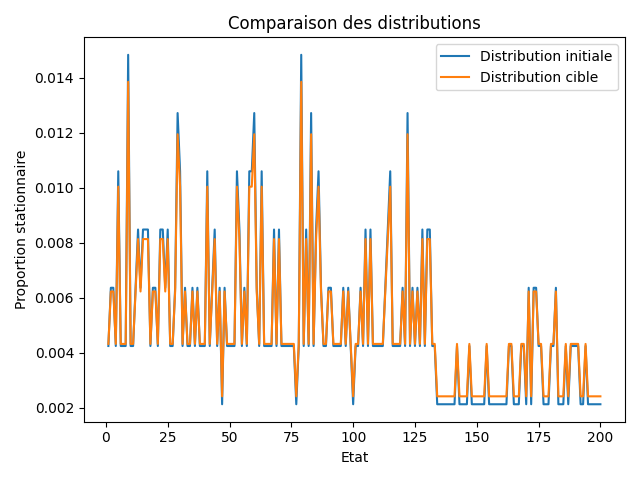
\includegraphics[width=.72\linewidth]{comparaison_distributions.png}
 \caption{Distributions initiale et cible pour \(\varepsilon=0{,}1\).}
 \label{fig:distributions}
\end{figure}
Le tableau~\ref{tab:transitions} montre les plus grandes modifications.
\begin{table}[htbp]
\centering
\begin{tabular}{lrrr}
\toprule
Transition & \(G_{ij}\) & \(\Delta^*_{ij}\) & \(\widehat G_{ij}\)\\
\midrule
Brenner \((64)\to\) Innsbruck \((63)\) & 0,5000 & \(-0,3130\) & 0,1870\\
Brenner \((64)\to\) Brenner \((64)\) & 0,0000 & \(+0,3130\) & 0,3130\\
Nagykanizsa \((120)\to\) Zagreb \((122)\) & 0,3333 & \(-0,2411\) & 0,0922\\
Maastricht \((4)\to\) Maastricht \((4)\) & 0,0000 & \(+0,2396\) & 0,2396\\
Maastricht \((4)\to\) Liège \((5)\) & 0,5000 & \(-0,2396\) & 0,2604\\
\bottomrule
\end{tabular}
\caption{Transitions les plus fortement modifiées.}
\label{tab:transitions}
\smallskip

Exemple : la probabilité d'aller de Brenner à Innsbruck diminue de
\(0{,}313\). Celle de rester à Brenner augmente de \(0{,}313\).
\end{table}

\section{Parcimonie}
On trouve \(265\) modifications non nulles sur \(672\) positions
autorisées. Le pourcentage est :
\[
 \frac{265}{672}\times100 \simeq 39{,}43\,\%.
\]
Donc \(60{,}57\,\%\) des positions autorisées ne changent pas. La
solution est relativement creuse : plus de la moitié des positions ne
changent pas. On compte aussi les positions diagonales.

La norme \(\ell_1\) favorise les solutions creuses. Mais elle ne garantit
pas le plus petit nombre possible de modifications.

\section{Sommet du polyèdre}
Un sommet est un « coin » du polyèdre des solutions admissibles.
On veut savoir si la solution trouvée par le solveur est un de ces coins.

\textbf{Critère du cours.} En forme standard, le polyèdre est
\[
 P=\{x:\mathcal A x=b,\ x\geq0\}.
\]
Pour une solution qui respecte les contraintes :
\begin{enumerate}
 \item On repère les variables positives dans \(x\).
 \item On garde les colonnes de \(\mathcal A\) liées à ces variables.
 \item Si ces colonnes sont indépendantes, la solution est un sommet.
\end{enumerate}
Par exemple, si \(x=(2,0,3)\), on garde les colonnes 1 et 3 : ce sont
les positions des valeurs positives. Pour tester l'indépendance, on
calcule le rang des colonnes gardées. Si le rang est égal au nombre de
colonnes, elles sont indépendantes.

\textbf{Avec notre solution, pour \(\varepsilon=0{,}1\) :}
\begin{enumerate}
 \item Le solveur donne une solution qui respecte les contraintes.
 \item On compte \(1322\) variables positives, avec le seuil \(10^{-9}\).
 \item On garde les \(1322\) colonnes correspondantes de \(\mathcal A\).
 \item Le calcul dans le code donne un rang de \(1322\).
\end{enumerate}
\[
 \text{rang }1322=\text{nombre de colonnes }1322.
\]
Les colonnes sont donc indépendantes à la précision du calcul près.
Notre solution est donc un sommet, d'après le critère du cours.
Le rang est calculé avec une tolérance numérique : le résultat est
donc vérifié à la précision de l'ordinateur près.

\section{Sensibilité à la cible}
On résout le problème pour cinq valeurs de \(\varepsilon\).
Pour chaque valeur, on note le coût et le nombre de modifications.
Une modification est comptée si sa valeur absolue dépasse \(10^{-9}\).
\begin{table}[htbp]
\centering
\begin{tabular}{rrr}
\toprule
\(\varepsilon\) & \(\sum_{(i,j)\in\Omega}|\Delta^*_{ij}|\) & Transitions modifiées\\
\midrule
0,05 & 6,0336 & 266\\
0,10 & 12,1383 & 265\\
0,25 & 31,8086 & 287\\
0,50 & 67,9718 & 321\\
0,75 & 99,1087 & 350\\
\bottomrule
\end{tabular}
\caption{Résultats de l'étude de sensibilité.}
\label{tab:sensibilite}
\end{table}
\begin{figure}[htbp]
 \centering
 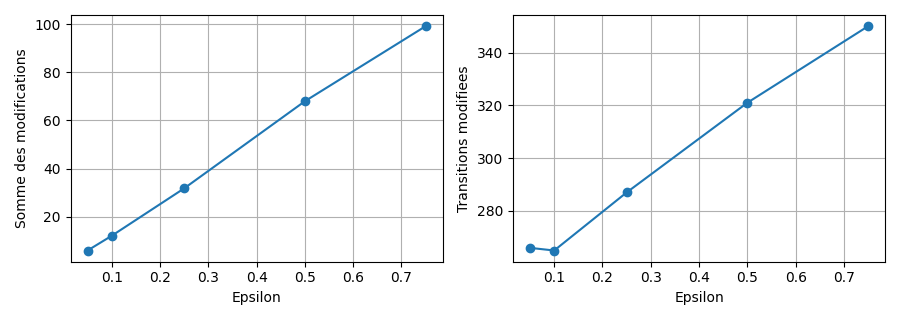
\includegraphics[width=.9\linewidth]{sensibilite_rapport.png}
 \caption{Coût optimal et nombre de transitions modifiées selon la cible.}
 \label{fig:sensibilite}
\end{figure}
\begin{itemize}
 \item Coût : \(6{,}0336\to99{,}1087\). Il augmente quand la cible
 devient plus uniforme.
 \item Nombre : \(266\to350\) globalement, mais \(266\to265\) entre
 \(0{,}05\) et \(0{,}10\).
 \item La somme mesure la taille des modifications, pas leur nombre.
 Ce nombre peut changer si on trouve une autre solution optimale.
\end{itemize}

\clearpage
\appendix
\section{Code de résolution}
Le fichier de données doit être à côté de \texttt{projet\_markov.py}. Pour enregistrer
la première figure, lancer le code depuis la racine du dépôt. Le code
calcule aussi les cinq résultats de sensibilité et enregistre leur figure.
\lstinputlisting[language=Python]{projet_markov.py}

\end{document}
